\documentclass[conference]{IEEEtran}
\IEEEoverridecommandlockouts
\renewcommand{\thesection}{\Roman{section}}
\usepackage{cite}
\usepackage{amsmath,amssymb,amsfonts}
\usepackage{booktabs}
\usepackage{array}
\usepackage{graphicx}
\usepackage{textcomp}
\usepackage{xcolor}
\usepackage{tikz}
\usetikzlibrary{positioning,arrows.meta,calc,fit,backgrounds}
\usepackage{pgfplots}
\pgfplotsset{compat=1.17}
\usepackage[ruled,vlined]{algorithm2e}
\usepackage{hyperref}
\hypersetup{colorlinks=true, linkcolor=blue!60!black,
            citecolor=blue!60!black, urlcolor=blue!60!black}

\pagestyle{empty}

\title{An Empirical Analysis of Entangled Enhancement in an Autonomous Driving Pipeline}

% \author{\IEEEauthorblockN{Rashedul Arefin Ifty, Fumio Machida}
% \IEEEauthorblockA{University of Tsukuba\\
% Tsukuba, Japan\\
% ifty.rashedul@sd.cs.tsukuba.ac.jp, machida@cs.tsukuba.ac.jp}}

\begin{document}
\maketitle
\thispagestyle{empty}
\bstctlcite{IEEEexample:BSTcontrol}% disable the dash for repeated author names

% ============================================================================
% STEP 1 SKELETON: every paragraph below is a planned topic sentence.
% Each topic sentence becomes one paragraph in Steps 2 to 6.
% ============================================================================

\begin{abstract}
Entangled enhancement is a defective retraining of a machine learning (ML) model that improves the updated model performance but fails to improve the whole system. No study has measured how often this effect occurs in a driving pipeline. This report empirically investigates entangled enhancement in an autonomous driving pipeline consisting of perception, prediction and planning modules. We examine whether an update that improves the perception model increases the error of the prediction and planning models, whether their adaptation to the errors of the perception model causes the increase, and whether entangled enhancement can be detected without ground truth. We train the prediction and planning models on the ground truth or on the output of the perception model before the update, keep both fixed, and update the perception model 30 times. We observe that the prediction error increases in 23 of 30 updates after training on the output of the perception model, in 11 by more than the change caused by a different random seed alone, and in 3 with statistical significance, against 5, 0 and 0 after ground-truth training. The planning error increases by at most 0.13\,m. As a result, we confirm that entangled enhancement occurs in the prediction model through its adaptation to the errors of the perception model. None of nine measures without ground truth identifies the updates with entangled enhancement.
\end{abstract}

\begin{IEEEkeywords}
autonomous driving, entangled enhancement, machine learning system, model maintenance, retraining
\end{IEEEkeywords}

% ============================================================================
\section{Introduction}
% ============================================================================

A Machine Learning System (MLS) is often built as a pipeline of ML models sequentially connected, where each model uses the output of the preceding model. A model earlier in the sequence is upstream, and a model later in the sequence is downstream. Retraining an upstream model can improve that model and still fail to improve the whole system. Wang and Machida call this effect entangled enhancement~\cite{wang2024compsac,wang2025issre}. Their work decides when an MLS should retrain each of its models. This decision needs the probability that a retraining causes entangled enhancement. No study has measured this probability on a real system.

A typical autonomous driving pipeline consists of three modules supported by machine learning (ML) models. The perception module finds the objects around the ego vehicle. The prediction module predicts where each object will move, and the planning module chooses the path of the ego vehicle.

Several studies describe the risk of entangled enhancement. Sculley et al.~\cite{sculley2015hidden} and Wu et al.~\cite{wu2021fixesthatfail} show that a change to one model of an MLS can make the whole system worse. Xu et al.~\cite{xu2024realworld} show that the prediction error increases when the input of the prediction model comes from a real perception model instead of the ground truth. None of these studies retrains the perception model of a driving pipeline and measures how often the error of the prediction and planning models increases, or which cause produces the increase.

In this report, we empirically investigate whether an update that improves the perception model increases the error of the prediction and planning models, and whether the increase comes from the adaptation of these models to the errors of the perception model. Adaptation means that the prediction and planning models, trained on the output of the perception model, learn to work with the errors of the perception model. We also examine whether entangled enhancement can be detected without ground truth. To separate the cause, we train the prediction and planning models either on the ground truth or on the output of the perception model before the update, keep both fixed, and update the perception model 30 times.

We observe that the prediction error increases in 23 of the 30 updates after training on the output of the perception model, and in 5 after training on the ground truth. As a result, we confirm that entangled enhancement occurs in the prediction model and comes from its adaptation to the errors of the perception model. The planning error increases by at most 0.13\,m. None of nine measures without ground truth identifies the updates with entangled enhancement.

% ============================================================================
\section{Background and Related Work}
% ============================================================================

This section summarises the related work.
Sculley et al.~\cite{sculley2015hidden} describe how a change to one model
of an MLS changes the behaviour of every model that uses the changed
output. Wu et al.~\cite{wu2021fixesthatfail} show that improving one model of a
system can make the whole system worse. In this report, we distinguish two causes of entangled enhancement. First, the downstream models adapt during training
to the errors of the upstream model and are disturbed when the retraining changes those
errors. Second, the upstream model improves on
average but becomes worse on the cases that matter downstream.

The prediction and planning models of this report follow two published models. AutoBot-Ego~\cite{girgis2022autobots} predicts the path of an object. PlanT~\cite{renz2022plant} plans the path of the ego vehicle from a list of objects. Weng et
al.~\cite{weng2022whose} show that a prediction model can learn by attention which of the objects found in different images are the same object. The prediction error increases
when the input comes from a real perception model instead of the ground
truth~\cite{xu2024realworld}. A planning model that receives
the state of the ego vehicle can score well on the nuScenes driving data set while ignoring the
objects~\cite{zhai2023rethinking,li2024egostatus}.

Rabanser et al.~\cite{rabanser2019failing} detect a change in the data seen by
a model without ground truth from distances between distributions, where a
distribution is the pattern of values that an output takes over many inputs.
In this report, we apply such distances to the outputs of the models as a candidate symptom, which is a sign of entangled enhancement that needs no ground truth.

% ============================================================================
\section{Methodology}
% ============================================================================

This section defines the target pipeline and the notation, and states the research questions and the hypotheses of this report.

\subsection{Target Pipeline and Notation}
This report focuses on an autonomous driving pipeline that consists of a perception module, a prediction module and a planning module. We write $C_1$ for the perception model, $C_2$ for the prediction model and $C_3$ for the planning model. $C_1$ finds the objects in the image of the front camera. $C_2$ predicts the path of each object over the next 3\,s. $C_3$ chooses the path of the ego vehicle over the same 3\,s. An update is one retraining of $C_1$ on new data. We write $C_1'$ for the updated $C_1$.

We write $\delta_1$ for the gain of $C_1$ in mAP50, the standard accuracy
measure for object detection. The prediction error is the minADE, which is the
average distance between the predicted path and the true path of an object,
taken for the best of the paths that $C_2$ predicts. The planning error is the
distance between the planned position and the position of the human driver at
3\,s. We write $\Delta_2$ and $\Delta_3$ for the increase of the prediction
error and of the planning error after an update. An update shows entangled
enhancement when
\begin{equation}
\delta_1 > 0 \quad \text{and} \quad (\Delta_2 > 0 \ \text{or} \ \Delta_3 > 0).
\label{eq:ee}
\end{equation}

\subsection{Research Questions and Hypotheses}
The goal of this report is to confirm whether entangled enhancement occurs in this pipeline, to find its cause, and to test whether it can be detected without ground truth. Each of the three research questions below leads to one hypothesis.

RQ1 asks whether an update that improves $C_1$ can increase the error of $C_2$ or $C_3$. The retraining decisions of Wang and Machida need the probability of this event, which no study has measured in a driving pipeline.

\noindent\textbf{H1 (an update that improves $C_1$ can increase the downstream error):} An update of $C_1$ can increase the prediction error or the planning error, even when the update makes $C_1$ more accurate.

RQ2 asks whether the increase comes from the adaptation of $C_2$ and $C_3$ to the errors of $C_1$. Only training on the output of $C_1$ lets $C_2$ and $C_3$ learn these errors, which the update then changes.

\noindent\textbf{H2 (the increase comes from the adaptation to the errors of $C_1$):} The increase is larger when $C_2$ and $C_3$ are trained on the output of $C_1$ than when $C_2$ and $C_3$ are trained on the ground truth.

RQ3 asks whether the updates with entangled enhancement can be detected without ground truth, because new data after deployment have no ground truth. A larger change in the output of $C_1$ or $C_2$ can cause a larger increase of the error.

\noindent\textbf{H3 (the updates with entangled enhancement change the outputs more):} An update with entangled enhancement changes the outputs of $C_1$ and $C_2$ more than an update without entangled enhancement. The gain $\delta_1$ alone does not indicate entangled enhancement.

% ============================================================================
\section{Experimental Setup}
% ============================================================================

This section presents the data set, the workflow of the experiment, and the ML models used for experiments. We ran all experiments in a Kaggle notebook with an Intel Xeon CPU at 2.0\,GHz (4 virtual cores), 31\,GB of RAM, Ubuntu 24.04 and two NVIDIA Tesla T4 GPUs with 15\,GB of memory each (Kaggle GPU T4 x2). Training used one of the two GPUs. The software is Python 3.13, PyTorch 2.11 with CUDA 12.8, and Ultralytics 8.4.

\subsection{Data}
We use 350 of the 850 scenes of nuScenes~\cite{caesar2020nuscenes},
which are driving clips of about 20\,s from Boston and Singapore, with the
full-size images of the front camera only (4.6\,GB). Boston~1 (100 scenes) trains $C_1$, and Boston~2 (100 scenes)
trains $C_2$ and $C_3$, with 14 of the scenes kept for validation. Separate scenes give $C_2$ and $C_3$ the realistic errors of $C_1$~\cite{xu2024realworld}. Singapore~1 (100 scenes) is used for the updates,
and Singapore~2 (50 scenes, 2{,}020 images) is used for testing. A keyframe is an image with labelled objects, recorded twice per second. The
test set has 1{,}720 test samples, one for every keyframe with 3\,s of
future.

\subsection{Workflow}
Fig.~\ref{fig:workflow} shows the six stages of the experiment. We split the data into four parts. Boston~1 and Boston~2 train the models, Singapore~1
provides the data for the updates, and Singapore~2 is the test set. We train
$C_1$ with two random seeds, where a random seed is the starting number
for the random choices made during training. We train $C_2$ and $C_3$ once in two training modes. In GT training, we train $C_2$ and $C_3$ on the ground truth (GT). In $C_1$-output training, we train $C_2$ and $C_3$ on the output of $C_1$. We then test each of the 30 updates in the full pipeline
with $C_2$ and $C_3$ kept fixed.

\begin{figure*}[t]
\centering
\resizebox{\textwidth}{!}{%
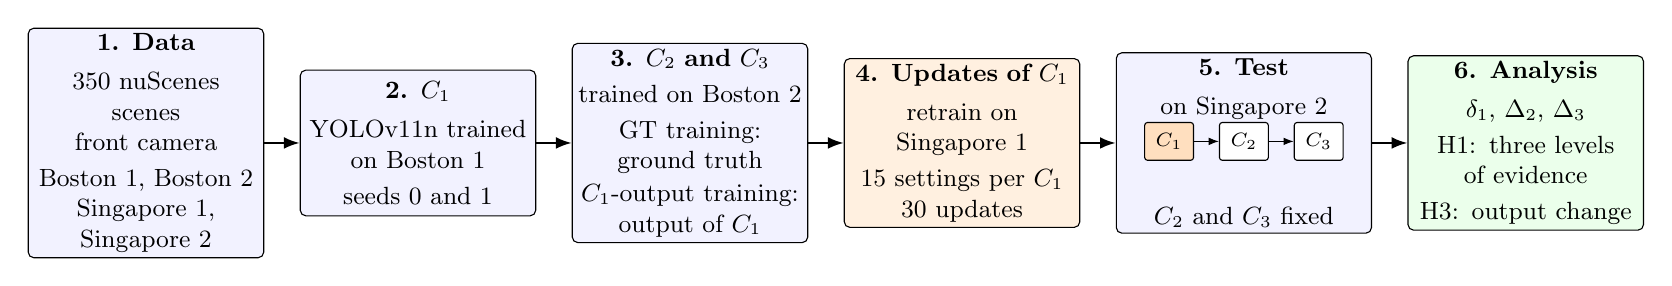
\begin{tikzpicture}[
  font=\small,
  stage/.style={draw, rounded corners=2pt, fill=blue!5, align=center,
                text width=2.85cm, minimum height=1.85cm, inner sep=2pt},
  head/.style={font=\small\bfseries, align=center},
  arr/.style={-{Latex[length=2mm]}, thick},
  mod/.style={draw, rounded corners=1pt, fill=white, minimum width=0.62cm,
              minimum height=0.48cm, inner sep=1pt, font=\scriptsize},
]
\node[stage] (s1) at (0,0) {\textbf{1. Data}\\[3pt] 350 nuScenes scenes\\ front camera\\[2pt] Boston 1, Boston 2\\ Singapore 1, Singapore 2};
\node[stage, right=0.45cm of s1] (s2) {\textbf{2. $C_1$}\\[3pt] YOLOv11n trained\\ on Boston 1\\[2pt] seeds 0 and 1};
\node[stage, right=0.45cm of s2] (s3) {\textbf{3. $C_2$ and $C_3$}\\[2pt] trained on Boston 2\\[2pt] GT training:\\ ground truth\\[1pt] $C_1$-output training:\\ output of $C_1$};
\node[stage, right=0.45cm of s3, fill=orange!12] (s4) {\textbf{4. Updates of $C_1$}\\[3pt] retrain on Singapore 1\\[2pt] 15 settings per $C_1$\\ 30 updates};
\node[stage, right=0.45cm of s4, text width=3.1cm] (s5) {\textbf{5. Test}\\[3pt] on Singapore 2\\[16pt] \phantom{x}\\[2pt] $C_2$ and $C_3$ fixed};
\node[stage, right=0.45cm of s5, fill=green!8] (s6) {\textbf{6. Analysis}\\[3pt] $\delta_1$, $\Delta_2$, $\Delta_3$\\[2pt] H1: three levels\\ of evidence\\[2pt] H3: output change};
\foreach \a/\b in {s1/s2,s2/s3,s3/s4,s4/s5,s5/s6} \draw[arr] (\a) -- (\b);
% small pipeline inside stage 5
\node[mod, fill=orange!25] (p1) at ($(s5.center)+(-0.95,0.02)$) {$C_1$};
\node[mod] (p2) at ($(s5.center)+(0,0.02)$) {$C_2$};
\node[mod] (p3) at ($(s5.center)+(0.95,0.02)$) {$C_3$};
\draw[-{Latex[length=1.3mm]}] (p1) -- (p2);
\draw[-{Latex[length=1.3mm]}] (p2) -- (p3);
\end{tikzpicture}}
\caption{Workflow of the experiment}
\label{fig:workflow}
\end{figure*}

\subsection{Update Procedure}
Algorithm~\ref{alg:campaign} gives the procedure for one $C_1$, where GT marks GT training and out marks $C_1$-output training. The two $C_1$ trained with seeds 0 and 1 have almost the same accuracy. Replacing one by the other still changes the errors of $C_2$ and $C_3$, although neither $C_1$ is better. We call the largest of these changes the seed variation, $\tau_2$ for the prediction error and $\tau_3$ for the planning error. An increase smaller than the seed variation can come from randomness alone. We count the increases at three levels of evidence. The first level counts any increase. The second level
counts an increase above the seed variation. The third level counts an
increase whose 95\,\% bootstrap interval lies above zero. The bootstrap
repeats the measurement on test sets drawn with replacement from the test
scenes.

\begin{algorithm}[t]
\footnotesize
\DontPrintSemicolon
\SetKwInOut{Input}{Input}\SetKwInOut{Output}{Output}
\Input{$C_1$, settings $\mathcal{S}$, Boston~2, Singapore~1, Singapore~2}
\Output{$\delta_1$, $\Delta_2$, $\Delta_3$ and evidence level per update and training}
Train $C_2^{\mathrm{GT}}, C_3^{\mathrm{GT}}$ on the ground truth of Boston~2\;
Train $C_2^{\mathrm{out}}, C_3^{\mathrm{out}}$ on the output of $C_1$ on Boston~2\;
\ForEach{training $r \in \{\mathrm{GT}, \mathrm{out}\}$}{ $E_2^{r}, E_3^{r} \leftarrow$ errors of $C_1 \rightarrow C_2^{r} \rightarrow C_3^{r}$ on Singapore~2\;
}
$\tau_2, \tau_3 \leftarrow$ seed variation from the $C_1$ with the other seed\;
\ForEach{setting $s \in \mathcal{S}$}{
  $C_1' \leftarrow$ retrain $C_1$ on Singapore~1 with $s$\;
  $\delta_1 \leftarrow \mathrm{mAP50}(C_1') - \mathrm{mAP50}(C_1)$\;
  \ForEach{training $r \in \{\mathrm{GT}, \mathrm{out}\}$}{ $\Delta_2, \Delta_3 \leftarrow$ errors of $C_1' \rightarrow C_2^{r} \rightarrow C_3^{r}$ minus $E_2^{r}, E_3^{r}$\;
    record the three levels of evidence\;
  }
  record the output change of $C_1$ and $C_2$ for H3\;
}
\caption{Update procedure for one $C_1$}
\label{alg:campaign}
\end{algorithm}


\subsection{Updates of the Perception Module}
We use YOLOv11n~\cite{jocher2024yolo11} as a perception model ($C_1$), which is trained for 10 passes over
Boston~1 with the random seeds 0 and 1. The two $C_1$ reach an mAP50 of
0.109 and 0.117 on Singapore~2. In each update, we retrain $C_1$ on Singapore~1
with one of 15 settings. Nine settings use 100\,\%, 50\,\% or 25\,\% of the images with 10 passes, and six use all images with 5 or 20 passes, each with the seeds 1, 2 and 3. The 15 settings
applied to both $C_1$ give 30 updates. The test scenes are never used to choose a model.

\subsection{ML Prediction and Planning Modules}
AutoBot-Ego~\cite{girgis2022autobots} is employed as a prediction model ($C_2$). For each current object,
a transformer reads the objects of the last four keyframes relative to that
object and outputs six possible paths of 3\,s, without a hand-written rule that links objects across images~\cite{weng2022whose}. For the planning model ($C_3$), we employ PlanT~\cite{renz2022plant}. Every object is one input with the current position, the most likely path from $C_2$, the class and the confidence. Two further inputs hold the driving command and the path of the ego vehicle over the last 1.5\,s, which we call the ego path. The command is left, straight or right~\cite{zhai2023rethinking}, and a recurrent decoder outputs six points of the planned path.

We train both models on Boston~2 with early stopping on the validation
scenes and with mirror and rotation augmentation. An input of the ego path can
let a planning module ignore the objects~\cite{li2024egostatus}, and we check whether $C_3$ uses the objects. Removing the objects from the input of $C_3$ moves the planned
position at 3\,s by 0.73 to 1.65\,m on average, which is above the threshold of
0.5\,m fixed before the experiment.

\subsection{Training and Measurements}
\label{sec:measures}
We train $C_2$ and $C_3$ once with GT training and once with $C_1$-output training for each $C_1$, and the trained models stay fixed during all updates. The prediction error is computed over the objects found by $C_1$ that are matched one to one with a ground truth object of the same class. The outputs of $C_2$ and
$C_3$ on the ground truth stayed exactly the same before and after every
update, which confirms that only the output of $C_1$ changed. The seed variation is $\tau_2 = 0.112$\,m and $\tau_3 = 0.018$\,m. For the bootstrap, we draw
the 50 test scenes 2{,}000 times with replacement.

% ============================================================================
\section{Results and Discussion}
% ============================================================================

In this section, we first check that $C_2$ and $C_3$ work, because a count of updates that increase the error is meaningful only for working modules. We then report and discuss the results. Every update made $C_1$ more accurate,
with $\delta_1$ between 0.048 and 0.118.

\subsection{Validity of the ML Components}
We compare $C_2$ and $C_3$ with simple baselines on the
test set (Table~\ref{tab:validity}). $C_2$ beats the baseline in which every object stays still. The variant of $C_3$ without the ego path does not beat the
baseline that drives the average Boston path for each command. We use the variant with the ego path, which has an error of 3.70 to 4.16\,m against 9.25\,m for the baseline.

\begin{table}[t]
\centering
\caption{ML models against simple baselines on the test set (m)}
\label{tab:validity}
\footnotesize
\setlength{\tabcolsep}{4pt}
\begin{tabular}{@{}lcc@{}}
\toprule
\textbf{Model and input} & \textbf{Model} & \textbf{Baseline} \\
\midrule
$C_2$ on the ground truth & 0.77 & 4.48 (stays still) \\
$C_2$ on the output of $C_1$ & 2.39 to 2.95 & 5.39 to 5.85 (stays still) \\
$C_3$ without the ego path & 9.3 to 12.5 & 9.25 (average path) \\
$C_3$ with the ego path & 3.70 to 4.16 & 9.25 (average path) \\
\bottomrule
\end{tabular}
\end{table}

\subsection{Prediction Module}
\label{sec:pred}
Fig.~\ref{fig:delta2} shows $\Delta_2$ for every update in two training modes. In all 30 updates, $\Delta_2$ after $C_1$-output training is larger than $\Delta_2$ after GT training. The
difference is largest for the updates from the $C_1$ with seed 0, where $\Delta_2$ after $C_1$-output training lies between $+0.049$ and $+0.284$\,m with a mean of $+0.165$\,m.

\begin{figure}[t]
\centering
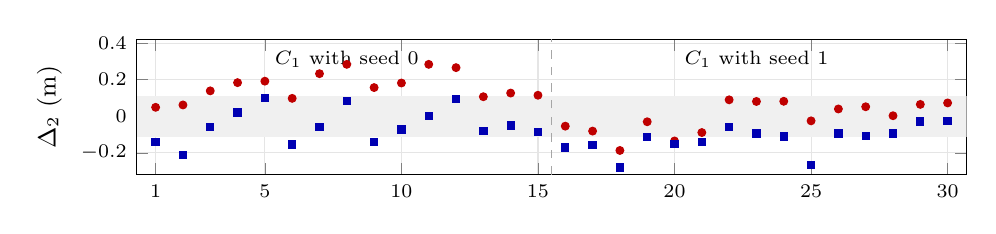
\begin{tikzpicture}
\begin{axis}[width=\columnwidth, height=3.3cm,
    ylabel={$\Delta_2$ (m)},
    xmin=0.3, xmax=30.7, ymin=-0.32, ymax=0.42,
    xtick={1,5,10,15,20,25,30}, tick label style={font=\scriptsize},
    label style={font=\small},
    grid=major, grid style={gray!20}]
\fill[gray!12] (axis cs:0.3,-0.112) rectangle (axis cs:30.7,0.112);
\draw[gray!70, dashed] (axis cs:15.5,-0.32) -- (axis cs:15.5,0.42);
\addplot[only marks, mark=*, mark size=1.4pt, color=red!75!black] coordinates {
(1,0.049) (2,0.062) (3,0.139) (4,0.184) (5,0.192) (6,0.098) (7,0.233) (8,0.284) (9,0.157) (10,0.182) (11,0.284) (12,0.266) (13,0.107) (14,0.127) (15,0.115) (16,-0.054) (17,-0.081) (18,-0.187) (19,-0.030) (20,-0.135) (21,-0.089) (22,0.090) (23,0.081) (24,0.082) (25,-0.025) (26,0.040) (27,0.052) (28,0.003) (29,0.065) (30,0.073)};
\addplot[only marks, mark=square*, mark size=1.3pt, color=blue!70!black] coordinates {
(1,-0.141) (2,-0.212) (3,-0.060) (4,0.021) (5,0.100) (6,-0.154) (7,-0.058) (8,0.082) (9,-0.141) (10,-0.073) (11,0.001) (12,0.093) (13,-0.079) (14,-0.051) (15,-0.085) (16,-0.170) (17,-0.156) (18,-0.280) (19,-0.115) (20,-0.152) (21,-0.141) (22,-0.059) (23,-0.095) (24,-0.111) (25,-0.267) (26,-0.094) (27,-0.107) (28,-0.094) (29,-0.029) (30,-0.025)};
\node[font=\scriptsize, anchor=north] at (axis cs:8,0.41) {$C_1$ with seed 0};
\node[font=\scriptsize, anchor=north] at (axis cs:23,0.41) {$C_1$ with seed 1};
\end{axis}
\end{tikzpicture}
\caption{$\Delta_2$ in the 30 updates. Red circles show $C_1$-output training, blue squares show GT training, and the grey band shows the seed variation.}
\label{fig:delta2}
\end{figure}

Table~\ref{tab:counts} counts the updates with an increase at the three levels
of evidence. We observe that, above seed variation, the prediction error increased in 11 updates after $C_1$-output training and in none after GT training. All 11 updates start from the $C_1$ with seed 0. With 50 test scenes, the bootstrap interval of $\Delta_2$ spans about $\pm 0.25$\,m. Only 3 updates after $C_1$-output training and none after GT training have an interval above zero.

The comparison results characterize the first cause of entangled enhancement. Both versions of $C_2$ receive the same output of $C_1'$. Only the version that learned from the output of $C_1$ becomes worse (Fig.~\ref{fig:delta2}).

\begin{table}[t]
\centering
\caption{Updates, out of 30, with an increase of the error}
\label{tab:counts}
\footnotesize
\setlength{\tabcolsep}{4pt}
\begin{tabular}{@{}lcccc@{}}
\toprule
& \multicolumn{2}{c}{\textbf{Prediction $\Delta_2$}} & \multicolumn{2}{c}{\textbf{Planning $\Delta_3$}} \\
\cmidrule(lr){2-3}\cmidrule(l){4-5}
\textbf{Level of evidence} & \textbf{$C_1$-output} & \textbf{GT} & \textbf{$C_1$-output} & \textbf{GT} \\
\midrule
Any increase & 23 & 5 & 18 & 29 \\
Above seed variation & 11 & 0 & 13 & 29 \\
Bootstrap interval above zero & 3 & 0 & 1 & 10 \\
\bottomrule
\end{tabular}
\end{table}

\subsection{Planning Module}
The planning error changed little. The mean $\Delta_3$ lies between $-0.006$
and $+0.058$\,m, and the largest value is 0.13\,m against a planning error of
about 4\,m. The increase appears more often after GT training than after $C_1$-output training at every level in Table~\ref{tab:counts}. Adaptation to the errors of $C_1$ cannot explain an increase after GT training.

$\Delta_3$ is small because $C_3$ plans mainly from the ego path. The objects move the planned position at 3\,s by only 0.73 to 1.65\,m.  The more frequent increase after GT training points to the second cause. The $C_3$ trained on the ground truth receives the predicted paths of $C_2$ only at test time. A change in the objects that $C_1'$ finds can therefore affect this $C_3$ more than the $C_3$ trained on the output of $C_1$.

\subsection{Retraining $C_2$ and $C_3$ on the Output of $C_1'$}
We test whether retraining $C_2$ and $C_3$ together with $C_1$ lowers the prediction error and the planning error below their values before the update. We retrain $C_2$ and $C_3$ on the output of $C_1'$ for two further updates, one from each $C_1$ with all images and 10 passes. After $C_1$-output training, the prediction error after the update is 2.75 and 2.61\,m, and the planning error is 4.14 and 4.00\,m. After the retraining, the prediction error is 2.39 and 2.45\,m, and the planning error is 3.71 and 3.70\,m.

The retraining lowers the prediction error by 0.36 and 0.16\,m and the planning error by 0.44 and 0.30\,m. The errors also fall below the errors before the update (2.62 and 2.66\,m, 4.16 and 4.00\,m), and the update becomes an improvement of the whole pipeline. This result supports the retraining of downstream models that Wang and Machida model~\cite{wang2024compsac,wang2025issre}. This retraining has a cost. A symptom of entangled enhancement is therefore useful.

\subsection{Symptom of Entangled Enhancement}
Nine measures of output change need no ground truth, seven on the output of $C_1$ and two on the output of $C_2$. The rank correlation with $\Delta_2$ is close to 1 when a larger measure always comes with a larger $\Delta_2$. The AUROC is the probability
that an update with $\Delta_2 > 0$ has a larger measure than an update with $\Delta_2 \le 0$. Over all 30 updates, the shift of the predicted position of the same
object has the highest rank correlation ($+0.68$, AUROC 0.81). For each
$C_1$ separately, the rank correlation is only $+0.29$ and $-0.28$. The high
value over all updates comes from the difference between the two $C_1$.
The gain $\delta_1$ has a rank correlation of $+0.04$. No measure consistently separates the updates that increase the prediction error from the other updates. H3 is therefore not supported.

% ============================================================================
\section{Conclusion}
% ============================================================================

In this report, we updated the perception module 30 times. We observe that the prediction module became worse more often and by more after $C_1$-output training than after GT training. This result
supports H1 and H2 for the prediction model and points to adaptation to the errors
of the perception model before the update as the cause. The planning error changed little.
No measure of output change that needs no ground truth identified the updates that increased the prediction error. H3 is therefore not supported. As future work, we develop a method that detects entangled enhancement after an update of the perception module, before the update is used and before ground truth for the new data exists.

\bibliographystyle{IEEEtran}
\bibliography{references}

\end{document}
